\documentclass{rapport}
\usepackage[utf8]{inputenc}

\usepackage{pifont} % Pour les symboles appelés par la macro \ding
\usepackage{url} % Comme son nom l'indique, pour les url...

\usetikzlibrary{positioning} % Bibliothèque tikz pour positionner des nœuds relativement à d'autres

\usepackage[colorlinks, citecolor=red!60!green, linkcolor=blue!60!green, urlcolor=magenta]{hyperref} % Pour que les liens soient cliquables. Les options permettent de mettre les liens en couleur.

\usepackage{algorithm}
\usepackage{algo}
\usepackage{colorationSyntaxique}


% Pour un rapport en français 
\usepackage[francais]{babel} % Commenter pour un rapport en anglais
\renewcommand\bibsection{\section*{Bibliographie}} % Commenter pour un rapport en anglais

% \englishTitlePage % Décommenter pour une page de titre en anglais


\pagestyle{fancy}
\renewcommand{\sectionmark}[1]{\markboth{\thesection.\ #1}{}}
\fancyfoot{}

\fancyhead[LE]{\textsl{\leftmark}}
\fancyhead[RE, LO]{\textbf{\thepage}}
\fancyhead[RO]{\textsl{\rightmark}}

\def\Latex{\LaTeX\xspace}
\def\etc{\textit{etc.}\xspace}


\title{Architecture des processeurs hautes performances}
\author{Ghizzardi, Enzo, Master 1 Informatique}
\supervisor{Sid, Touati}
\date{1e semestre de l'année 2024-2025}

% \universityname{Université Côte d'Azur} % Nom de l'université.
% \type{Projet} % Type de document
% \formation{Master Informatique} % Nom de la formation

% Retrouver les autres options possibles dans le document rapport.pdf

\begin{document}

  \maketitle

  \begin{abstract}
    Dans le cadre de ce projet, nous explorons les performances des processeurs modernes à travers l’étude approfondie de leur hiérarchie mémoire. Cette hiérarchie, composée de multiples niveaux de cache et de la mémoire principale, joue un rôle déterminant dans l’efficacité des applications informatiques. Grâce à des exercices pratiques et des outils de benchmarking, le projet vise à répondre à une problématique centrale : comment optimiser l’accès aux données dans des systèmes à mémoire multi-niveaux pour maximiser les performances ?\\[1mm]
    
    Trois axes principaux sont abordés dans ce rapport. Tout d’abord, une analyse des temps d’accès aux caches (Exercice 1) permet d’identifier les seuils critiques liés aux tailles des données. Ensuite, une évaluation de la bande passante mémoire (Exercice 2) met en évidence les limites du transfert de données entre le processeur et la mémoire centrale. Enfin, l’utilisation de l’outil \textbf{Calibrator} (Exercice 5) apporte une vision détaillée des performances des caches en fonction de différents paramètres, tels que la taille des plages et le pas d’accès.\\[1mm]
    
    Ce travail s’appuie sur une méthodologie rigoureuse, incluant la configuration minimale d’un système Linux et l’emploi de micro-benchmarks développés en langage C. Les résultats obtenus offrent des perspectives précieuses pour mieux comprendre les interactions entre matériel et logiciel, tout en ouvrant des pistes pour le développement d’applications plus performantes et adaptées aux architectures modernes.\\[1mm]
  \end{abstract}

  \clearpage
  \tableofcontents

  \clearpage

  %%%%%%%%%%%%%%%%%%%%%%%%%
  % Consignes et conseils %
  %%%%%%%%%%%%%%%%%%%%%%%%%

    \section{Introduction}
    
        Ce rapport présente le travail effectué sur trois exercices de TP ayant pour objectif d'évaluer les performances de la hiérarchie mémoire d’une machine. Le but était de faire une analyse des caches de divers niveaux, de la mémoire centrale ou encore de la bande passante à l'aide de benchmarks programmé en C et d'autres outils.
        Nous allons dans un premier temps détailler l'environnement expérimentale ainsi que la configuration de la machine durant les expériences.
        Nous parcourerons ensuite les différents exercices de ce TP en détaillant la démarche et en analysant les résultats.
        Nous pourrons enfin faire quelques remarques pertinentes et conclure sur ce petit projet.
        Ce document retrace les étapes principales de cette étude, les méthodes utilisées, et les enseignements tirés des résultats.
        
    \section{Environnement expérimentale} 
      
      \subsection{Environnement matériel} 
        La machine sur laquelle les benchmark ont été effectué est équipée d’un processeur \textbf{Intel 12th Gen Core i5-12600KF}. Voici les caractéristiques détaillées de l’architecture et de la micro-architecture de ce processeur, ainsi que des informations sur la hiérarchie mémoire.
        
        \begin{enumerate}
          \item \textbf{Processeur :}

            \begin{itemize}
                \item \textbf{Modèle :} Intel 12th Gen Core i5-12600KF,
                \item \textbf{Micro-architecture :} Alder Lake, qui combine des cœurs Performance (P-cores) pour des tâches exigeantes et des cœurs Efficient (E-cores) pour des tâches légères,
                \item \textbf{Cœurs et threads :}
                    \begin{itemize}
                        \item \textbf{Cœurs physiques :} 10 (6 cœurs Performance [P-cores] et 4 cœurs Efficient [E-cores]),
                        \item \textbf{Threads logiques :} 16 (grâce à la technologie Hyper-Threading activée sur les P-cores).
                    \end{itemize}
                \item \textbf{Fréquence d’horloge :}
                    \begin{itemize}
                        \item Base : 3.7 GHz,
                        \item Boost : Jusqu’à 4.9 GHz.
                    \end{itemize}
                \item \textbf{Pipeline :}
                    \begin{itemize}
                        \item Les P-cores disposent d’un pipeline à 19 étages optimisé pour des performances élevées,
                        \item Les E-cores disposent d’un pipeline simplifié pour une efficacité énergétique maximale,
                    \end{itemize}
                \item \textbf{Parallélisme :}
                    \begin{itemize}
                        \item Supporte le parallélisme d’instructions avec un mécanisme Out-of-Order (ROB de 512 entrées).
                    \end{itemize}
            \end{itemize}
          
          \item \textbf{Hiérarchie mémoire :}

            \begin{itemize}
                \item \textbf{Caches :}
                    \begin{itemize}
                        \item Cache L1 : 48 Ko pour les instructions et 32 Ko pour les données (par cœur),
                        \item Cache L2 : 1.25 Mo par cœur,
                        \item Cache L3 : 20 Mo partagé entre tous les cœurs (P-cores et E-cores).
                    \end{itemize}
                \item \textbf{Tailles des lignes de cache :} 64 octets pour tous les niveaux de cache,
            \end{itemize}
          
          \item \textbf{Autres caractéristiques matérielles :}

            \begin{itemize}
                \item \textbf{Extensions vectorielles :} Prend en charge AVX2, FMA, et AVX-VNNI,
                \item \textbf{Technologies supplémentaires :} Intel VT-x, Intel VT-d pour la virtualisation.
            \end{itemize}
          
        \end{enumerate}
        
      
      \subsection{Environnement logiciel} 
        \begin{enumerate}
          \item \textbf{Système d’exploitation :}

            \begin{itemize}
                \item \textbf{Distribution :} Fedora Linux 41 (Workstation Edition),
                \item \textbf{Version du noyau :} Linux 6.12.4-200.fc41.x86\_64,
                \item \textbf{Version du micrologiciel :} 4.02.
            \end{itemize}
            
          \item \textbf{Compilateur :}

            \begin{itemize}
                \item \textbf{Nom :} GNU Compiler Collection (GCC),
                \item \textbf{Version :} 12.3.1,
                \item \textbf{Options de compilation :}

                    \begin{itemize}
                        \item \verb:-O2: : Optimisation intermédiaire pour équilibrer performances et temps de compilation,
                        \item \verb:-march=native: : Génération de code optimisé pour l’architecture matérielle spécifique,
                    \end{itemize}
                
            \end{itemize}
          \item \textbf{Outils de mesure} :
            \begin{itemize}
                \item \textbf{Fonctions utilisées pour le chronométrage :}

                    \begin{itemize}
                        \item \verb:gettimeofday: : Fournit une précision en microsecondes pour les mesures temporelles,
                    \end{itemize}
            \end{itemize}
          
        \end{enumerate}

    \section{Configuration de la machine pendant les expériences} 
      
      \subsection{Processus et services actifs}
        Lors des tests, ma machine était configuré dans un environnement uniquement en ligne de commandes sur une console shell, sans interface graphique, où le plus de processus possibles ont été désactivé pour ne laisser que l'essentiel et éviter les parasites.
        Voici une liste des processus en activité sur ma machine lors des tests :

        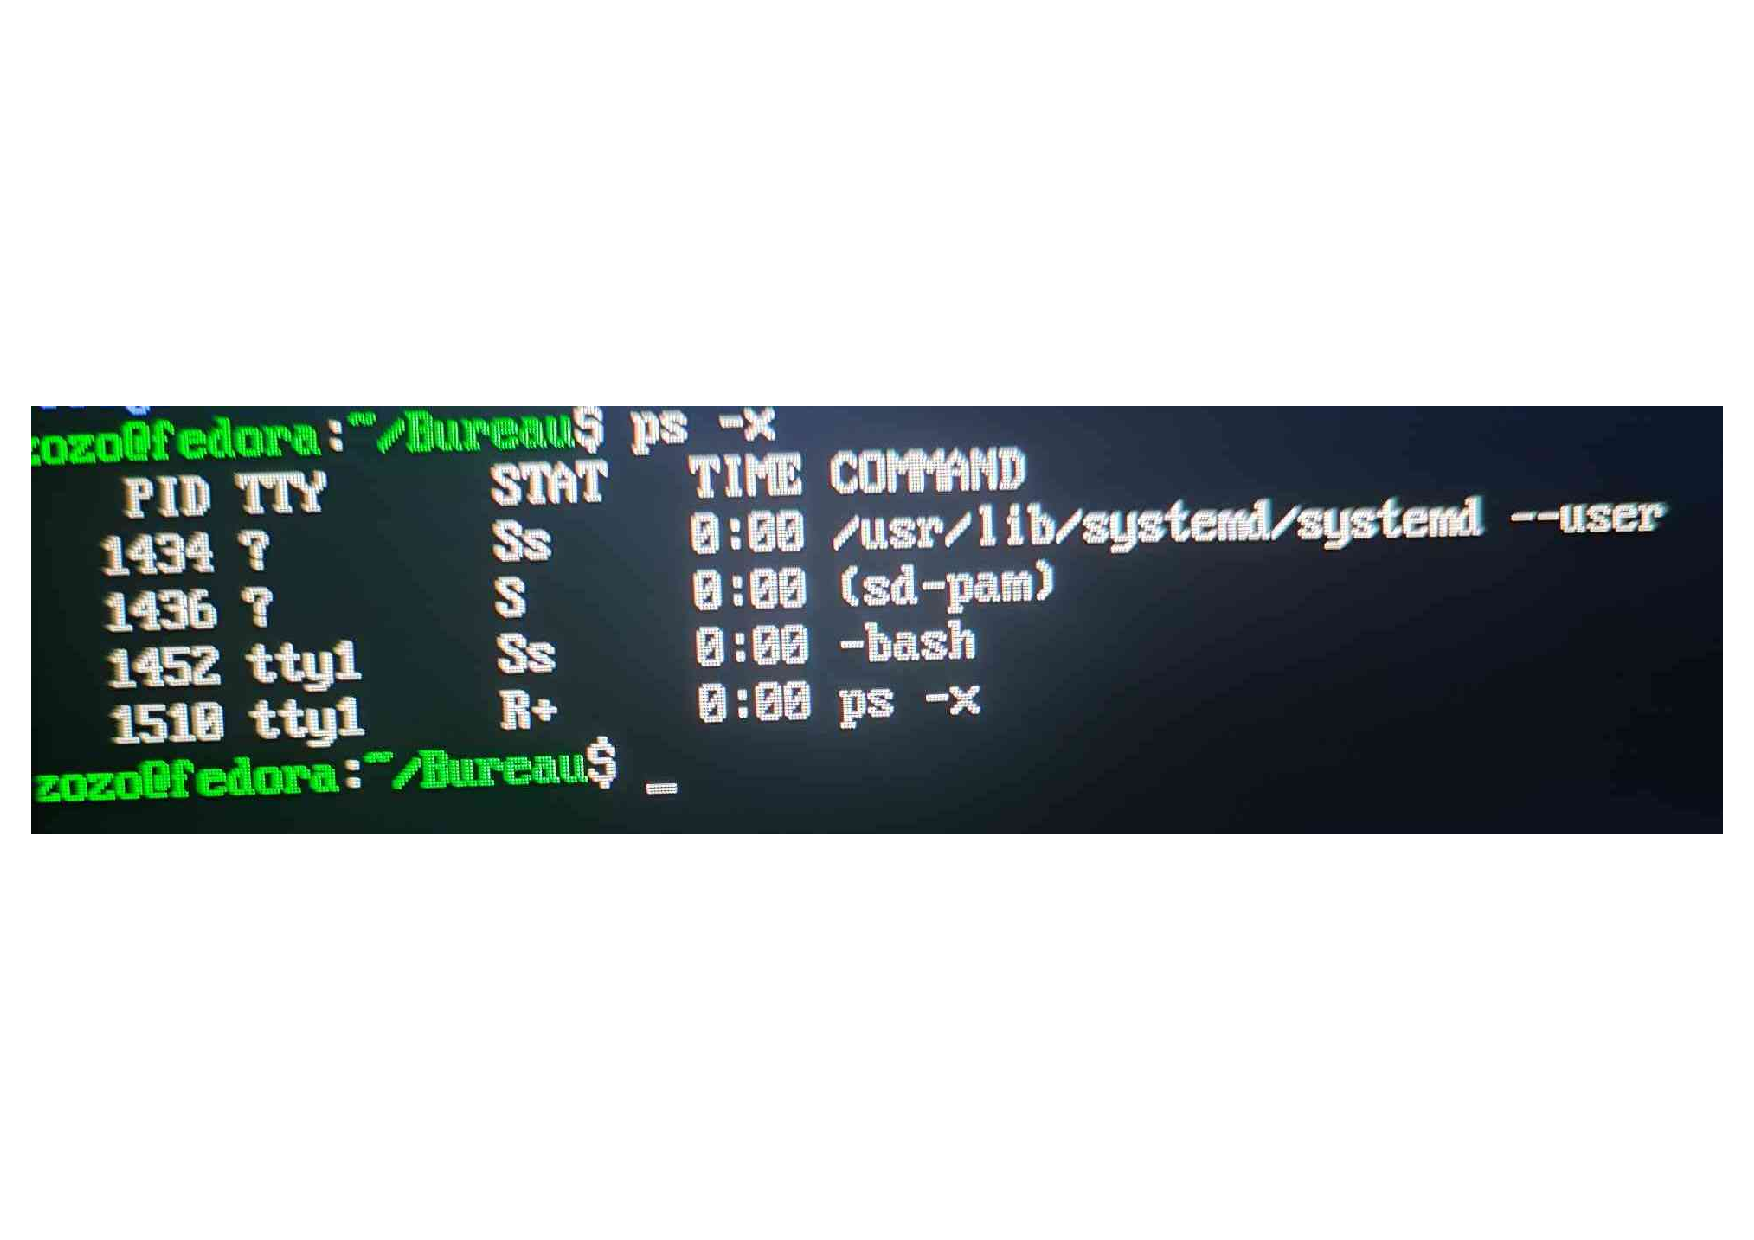
\includegraphics[width=15cm]{img/processus_actifs.pdf}

        Voici un détail de ces processus :
        
        \begin{itemize}
            \item \verb:/usr/lib/systemd/systemd --user: : C'est une instance utilisateur de \verb:systemd:, le système d'initialisation qui gère les services et sessions pour cet utilisateur. Ce processus est lancé pour configurer et gérer les services spécifiques à l'utilisateur ;
            \item \verb:(sd-pam): : PAM (Pluggable Authentication Modules) est utilisé pour gérer les sessions utilisateur, notamment pour l'authentification et les paramètres de session. Ce processus est une sous-composante de \verb:systemd --user: ;
            \item \verb:-bash: : C'est une session du shell \textbf{Bash}, qui est en cours d'exécution dans le terminal virtuel \verb:tty1:. Le \verb:-: indique qu'il s'agit d'un shell de connexion (login shell), chargé avec des variables d'environnement spécifiques ;
            \item \verb:ps -x: : C'est le processus correspondant à la commande que vous avez exécutée pour obtenir cette liste. Le processus est actif pendant que la commande est en cours d'exécution.
        \end{itemize}
      
      \subsection{Méthodologie de collecte des données}
      Les micro-benchmarks ont été exécutés dans un environnement en ligne de commande, directement accessible via une console shell. La collecte des données expérimentales s’est faite comme suit :
        \begin{itemize}
          \item Préparation des données : Chaque test a été exécuté plusieurs fois pour obtenir des résultats stables et reproductibles. Les temps d’accès ont été mesurés avec la fonction \verb:gettimeofday:,
          \item Configuration spécifique : Les paramètres des benchmarks ont été ajustés pour évaluer différents niveaux de la hiérarchie mémoire. Par exemple, la taille des tableaux accédés a été progressivement augmentée pour détecter les limites des caches,
          \item Enregistrement des résultats : Les résultats ont été enregistrés sous forme de fichiers tabulés, puis transformé en graphe à l'aide de gnuplot pour mieux lire les informations.
        \end{itemize}

  %%%%%%%%%%%%%%%%%%%%%%%%%
  % Exercices              %
  %%%%%%%%%%%%%%%%%%%%%%%%%

    \section{Exercice 1 - Tester les performances de la hiérarchie mémoire d’un CPU avec un micro-benchmark séquentiel}

    L’objectif de cet exercice est d’évaluer les performances de la hiérarchie mémoire d’un processeur en mesurant les temps d’accès moyens à différentes tailles de données. Cela permet de détecter les tailles des caches (L1, L2, L3) ainsi que la limite au-delà de laquelle les données doivent être chargées depuis la mémoire principale, ce qui impacte les performances.

    J'ai obtenue différents graphes. Certains exécutés sur un coeur précis, d'autres sans la précision \verb:taskset -c 0:. Certains avec 1 seule répétition, d'autres avec 10 répétitions. Voici ces différents résultats.

    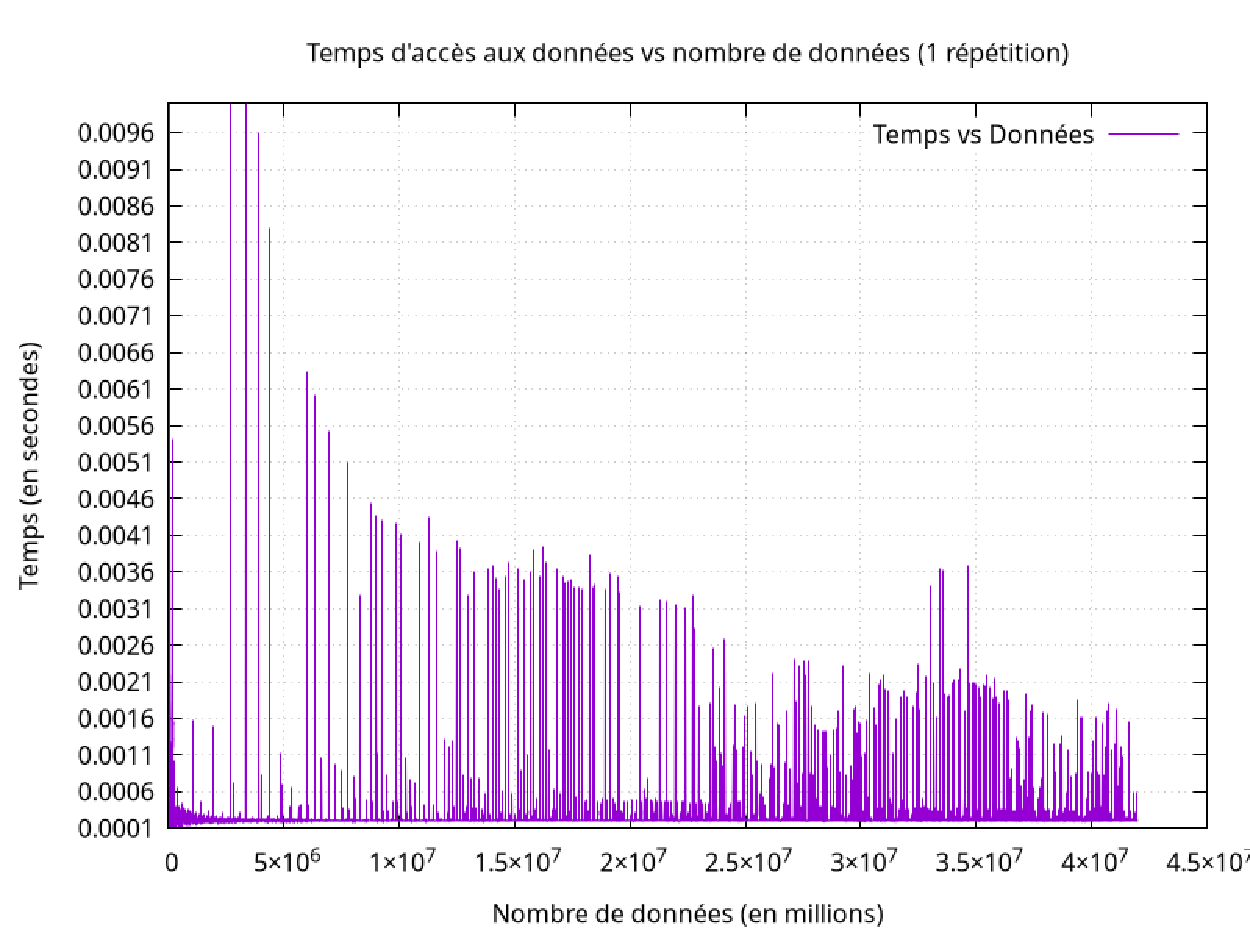
\includegraphics[width=13cm]{img/graphrep1.pdf} \\[1mm]
    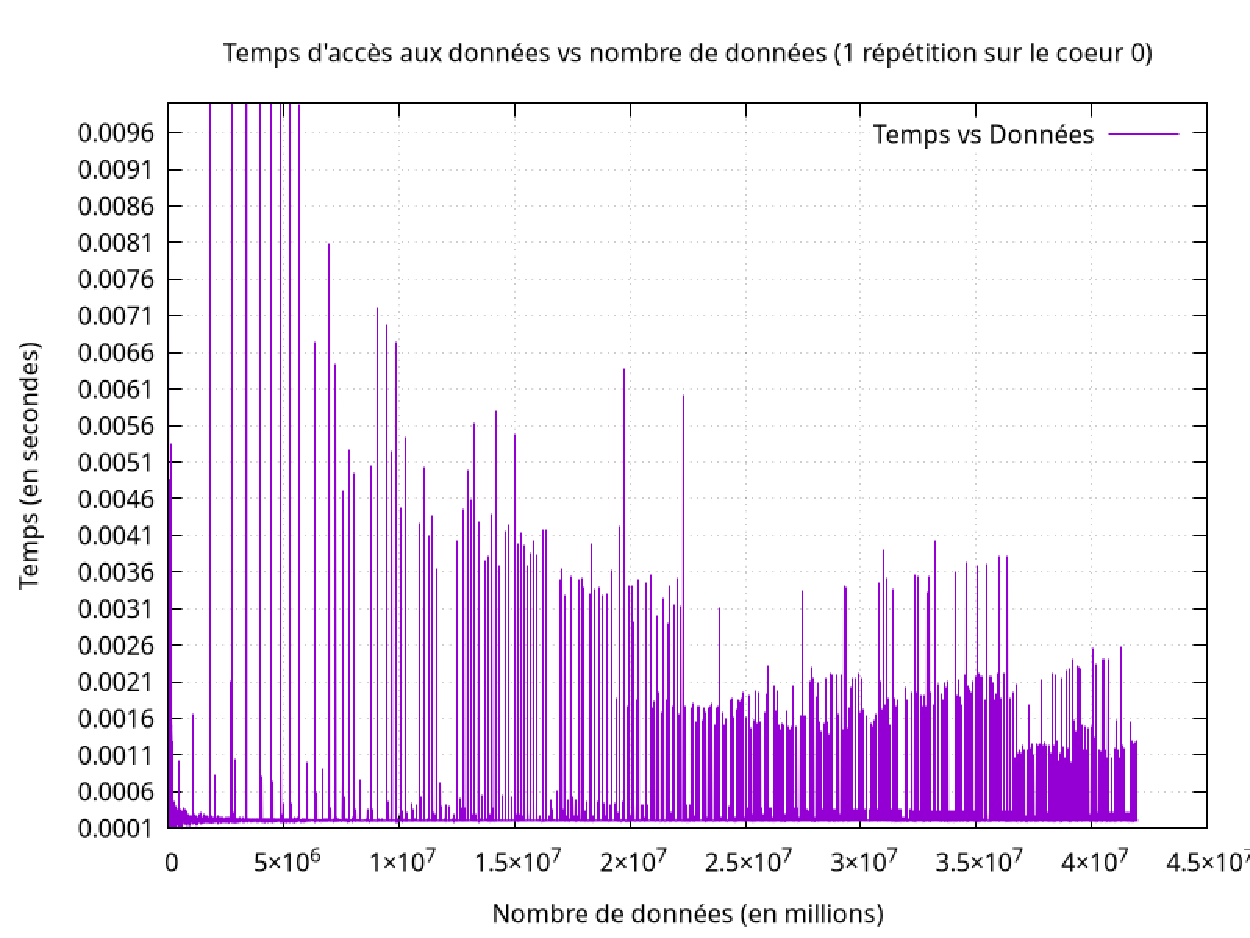
\includegraphics[width=13cm]{img/graphrep1core.pdf} \\[1mm]
    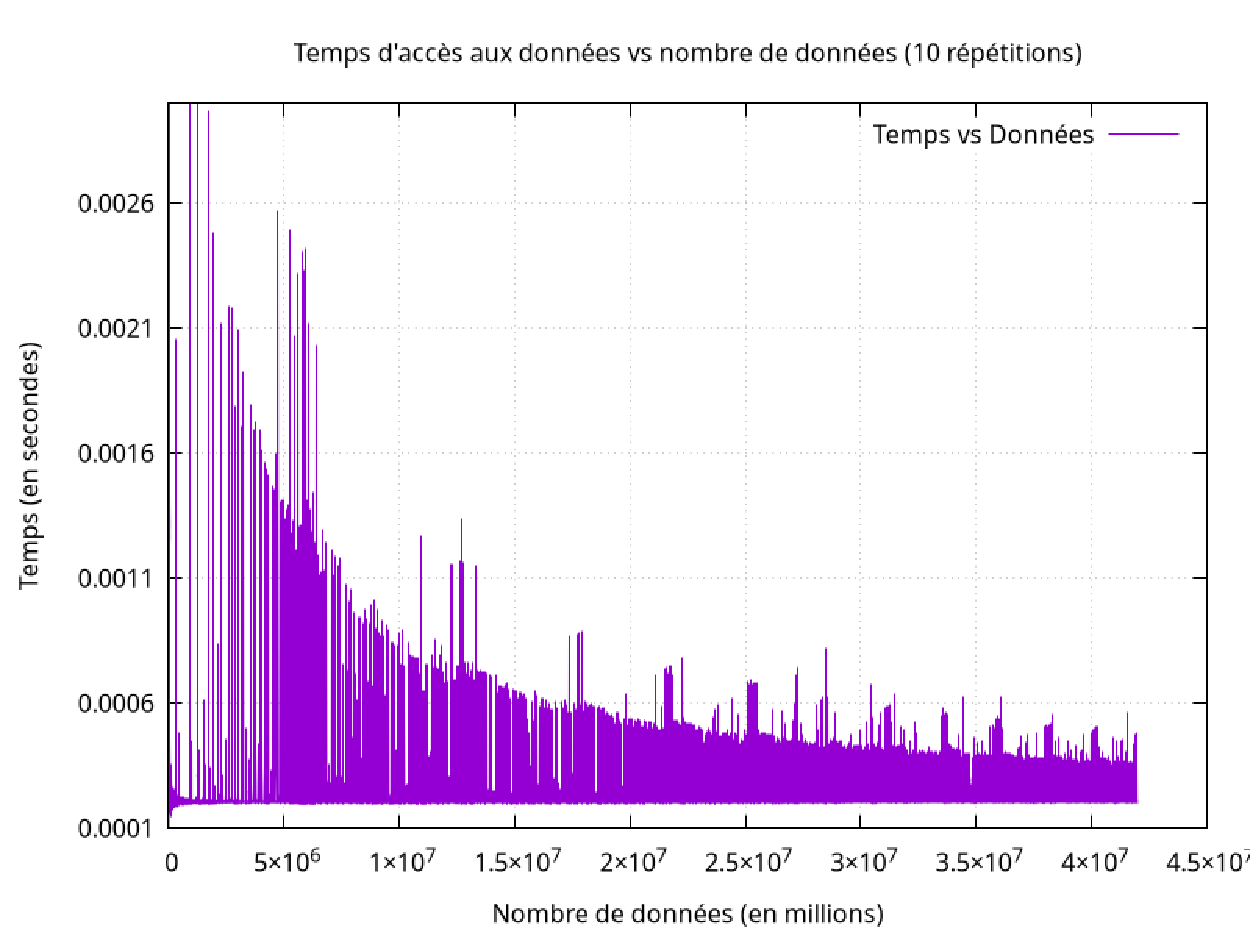
\includegraphics[width=13cm]{img/graphrep10.pdf} \\[1mm]
    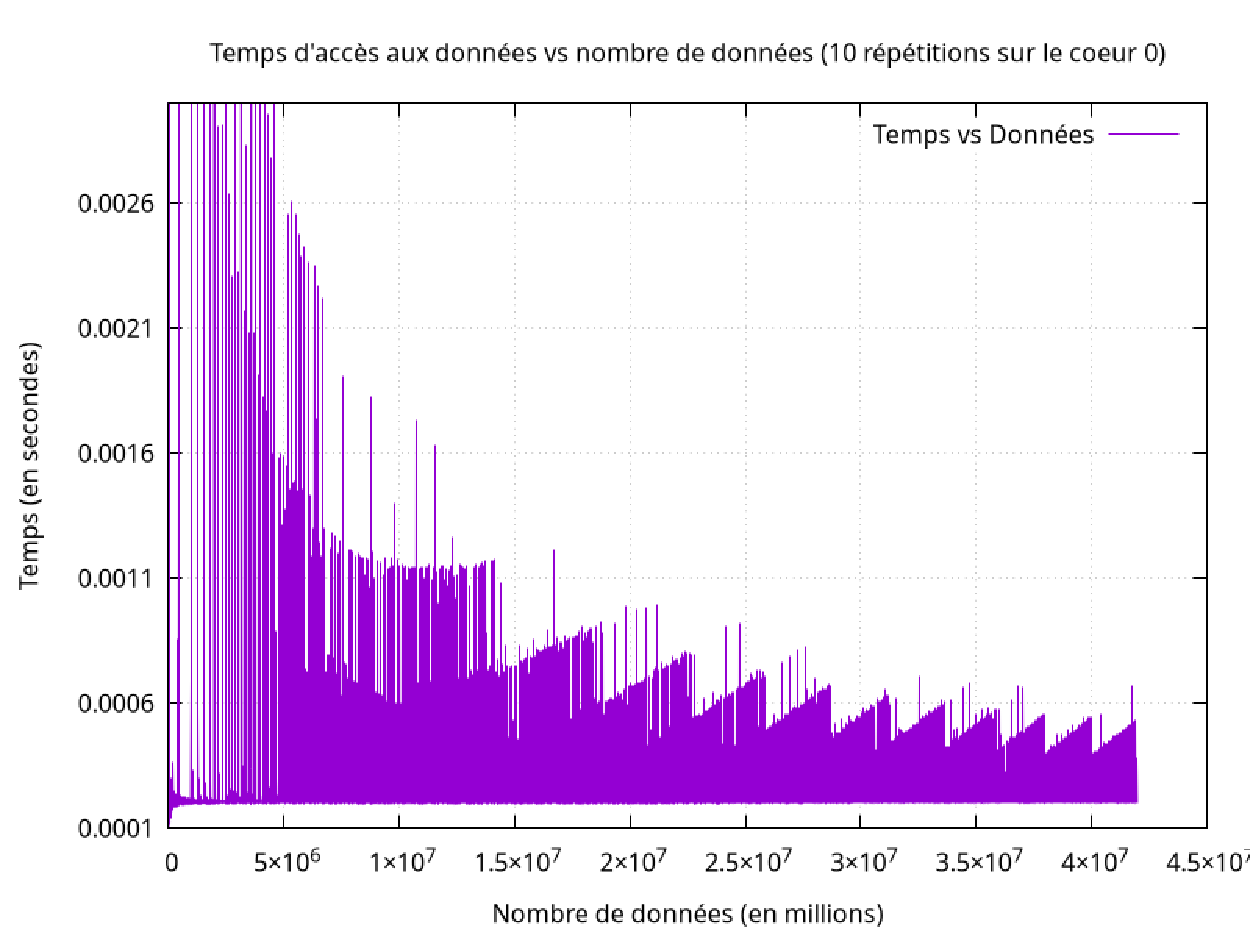
\includegraphics[width=13cm]{img/graphrep10core.pdf} \\[1mm]
    
    Etrangement, on remarque que les temps d'accès aux données diminuent avec le temps. On a également beaucoup de mal à réellement distinguer les palier qui représenteraient les différents caches sur ces graphes.

    Cela est peut-être due à des optimisations internes du processeur (préchargement, ordonnancement d’instructions) qui fausserait les résultats.

    \section{Exercice 2 - Évaluation de la bande passante entre le processeur et la mémoire centrale}

        Cet exercice vise à mesurer la bande passante effective entre le processeur et la mémoire centrale (RAM). La bande passante est une métrique clé pour évaluer la capacité du système à transférer efficacement des données entre le CPU et la mémoire, particulièrement dans des scénarios où les données dépassent la capacité des caches.
        
        \subsection{Méthodologie}

            Pour estimer la bande passante entre le processeur et la mémoire centrale, on doit connaitre le temps moyen d'accès à la mémoire. Il faut également savoir la taille du cache L3 et celle des lignes de cache pour déterminer la taille du tableau, ainsi que le pas nécessaire pour éviter que des données soient préchargées en mémoire. Pour cela, il est conseillé de choisir une taille de tableau équivalente à deux fois la taille du cache L3, ainsi qu’un pas suffisamment grand pour dépasser les mécanismes de préchargement matériel et de mise en cache. Sur ma machine, le cache L3 a une taille de 20 Mo, ce qui correspond à (2 * 20 * 1024 * 1024) / sizeof(int), soit 10 485 760 éléments. En ce qui concerne le pas, on opte pour différentes valeurs, plus ou moins élevées, (2, 4 ou 8 fois la taille d’une ligne de cache). Des valeurs de pas élevées garantissent qu’aucune donnée ne soit préchargée. \\[2mm]

            \subsection{Résultats}

            Voici les résultats obtenues pour les différentes valeurs de multiplicateurs de pas :
            
            \begin{itemize}
            \item Pour un multiplicateur de pas de 2, nous avons un temps d'accès moyen de 67.291260 nanosecondes et une bande passante de 907.029480 Mo/s,
            \item Pour un multiplicateur de pas de 4, nous avons un temps d'accès moyen de 282.714844 nanosecondes et une bande passante de 215.889465 Mo/s,
            \item Enfin, pour un multiplicateur de pas de 8, nous avons un temps d'accès moyen de 1665.234375 nanosecondes et une bande passante de 36.652592 Mo/s.
            \end{itemize}
            Comme pouvant être observé dans les résultats en archives, il se passe des choses intéressantes lorsque l'on répète plusieurs fois de suite le benchmarK. Pour le benchmark avec un multiplicateur de pas de 2, le temps d'accès semble diminuer au file des répétitions (et le débit lui augmente).
            Pour ceux avec un multiplicateur de pas de 4 et 8, c'est beaucoup plus aléatoire. Au file des répétitions, les valeurs varient assez significativement.
            On observe également que l’augmentation du pas entraîne une augmentation du temps d’accès moyen à la mémoire.
            
    \section{Exercice 5 - Micro-benchmark plus sophistiqué : l’outil Calibrator}
      
      \subsection{Calibrator}
        
        Cet exercice consiste à utiliser l'outil "Calibrator" pour analyser les performances de la hiérarchie mémoire d’un processeur. L’objectif est d’identifier les tailles et les latences des différents niveaux de cache (L1, L2, L3) ainsi que d’évaluer la bande passante et la latence de la mémoire principale. En analysant le code, on comprend que le programme effectue des tests itératifs en parcourant des plages mémoire avec des pas croissants, permettant d’identifier les "paliers" de performances correspondant aux différents niveaux de cache.
        Il mesure précisemment le temps d'accès moyen (en cycles et en nanosecondes par itération), ainsi que la bande passante effective pour chaque combinaison de taille de pas.

      \subsection{Difficultés rencontrées}

        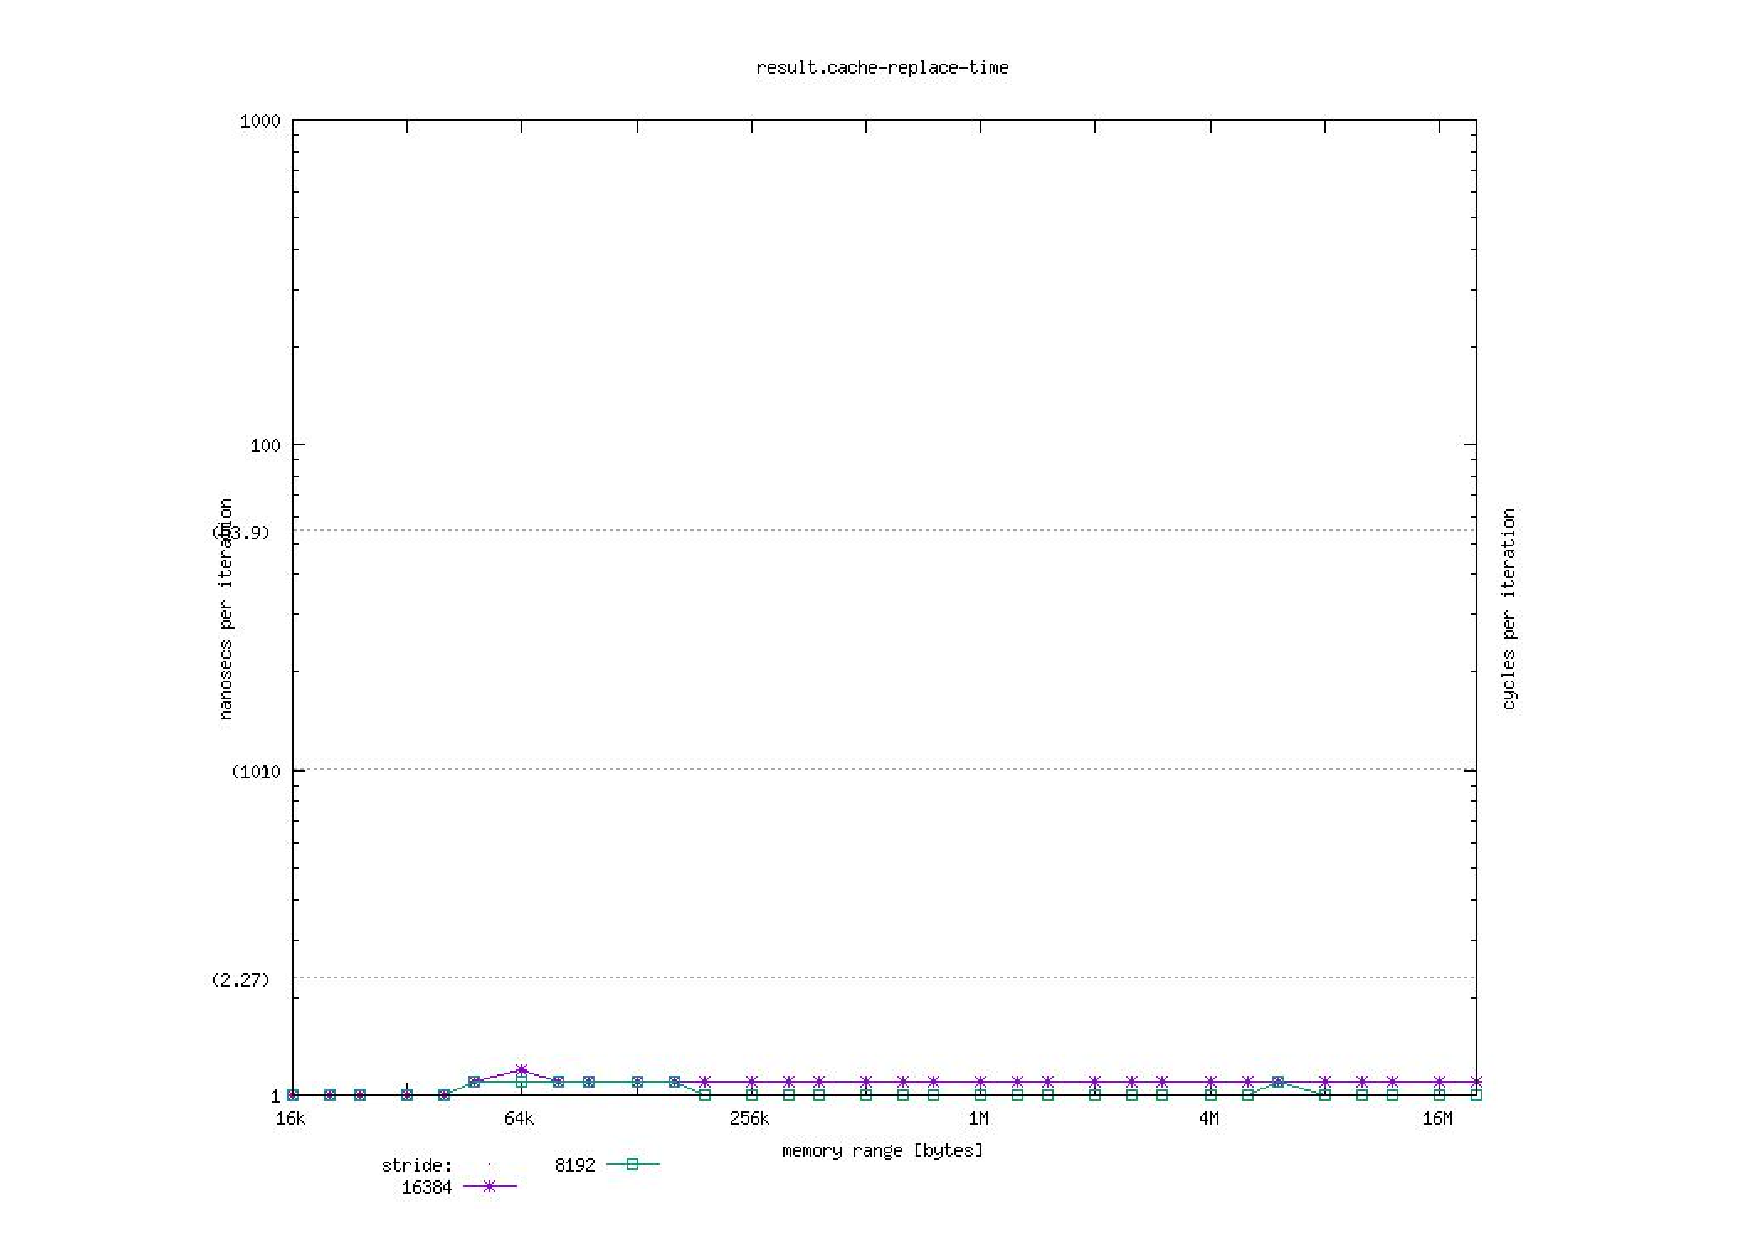
\includegraphics[width=15cm]{img/result.cache-replace-time.pdf}

        Je n'ai hélas jamais réussi à faire correctement fonctionner le calibrator sur ma machine. Le fichier se compile bien mais le fichier .gp renvoyé est incomplet et me permet seulement d'obtenir ce début de graphe.
        
            
        \section{Conclusion}

    Ce projet m'a permis d’approfondir la compréhension de la hiérarchie mémoire et des performances des processeurs modernes à travers des expérimentations pratiques. Les différents exercices réalisés ont mis en évidence les interactions complexes entre les niveaux de cache, le processeur, et la mémoire centrale.\\[2mm]
    L'analyse de l’\textbf{Exercice 1} nous a appris que la hiérarchie mémoire, avec ses différents niveaux de cache (L1, L2, L3), influence considérablement les performances. Le temps d'accès moyen augmente à mesure que la taille des données dépasse les capacités des caches, forçant le processeur à accéder à des niveaux de mémoire plus lents. Cependant, des anomalies dans les temps mesurés (diminution inattendue) ont mis en évidence des optimisations internes du processeur (préchargement, ordonnancement d’instructions), nécessitant des ajustements méthodologiques pour obtenir des résultats fiables.\\[2mm]
    L’\textbf{Exercice 2} a fourni une estimation précise de la bande passante entre le processeur et la mémoire principale, soulignant les limites physiques imposées par l’architecture matérielle. La bande passante mémoire effective dépend fortement de la taille des données et du pas d'accès. En accédant à des données non contiguës, nous avons simulé des scénarios où les caches sont sous-utilisés, forçant l'accès direct à la mémoire principale. Les techniques pour mesurer la bande passante, comme l'utilisation d'un pas important et la configuration minimale du système, ont renforcé l'idée que les tests doivent être soigneusement conçus pour éviter les biais.\\[2mm]
    Je n'ai hélas pas réussi à exécuter correctement le Calibrator de l’\textbf{Exercice 5}, mais cet outil offre une analyse plus détaillée que les micro-benchmarks développés dans les exercices précédents, permettant de caractériser précisément les tailles des caches, leurs latences d'accès, et les performances des TLBs (Translation Lookaside Buffers). L’utilisation d’un pas (stride) variable dans les tests permet de détecter des comportements subtils, comme les optimisations liées au préchargement matériel.\\[2mm]
    Ces résultats montrent que la performance d’un système informatique dépend non seulement de la puissance brute du processeur, mais aussi de la manière dont les données sont gérées dans la mémoire. Il est absolument nécessaire de mieux comprendre et apprivoiser ces méchanismes pour le développement d’applications plus performantes et plus adaptées à l’architecture.\\[2mm]

    
\end{document}
Ghizzardi